\chapter{Data Cubes}

While relational databases with highly normalized data models fit well to situations where data is frequently modified, they can be quite cumbersome when being performed complex aggregating queries. Online Analytical Processing (OLAP) system fits better these purposes. In an OLAP system, numerical data is stored in a multidimensional data structure. The structure is comprised of hypothetical cells, which are identified by their assigned set of dimension values from each dimension of the structure. Each cell can contain zero to many numerical values, so-called measurements. The structure is referred to as OLAP Cube or Data Cube. The word \textit{cube} implies exactly three dimensions, but its purpose is only to illustrate the multidimensionality of the structure.

Distinct values of a dimension can be organized into a hierarchy, where a parent value is assigned to summarized measurements throughout its child values. An example of such a hierarchy could be a relationship of a product category and specific products belonging to this category. The depth of a dimension value in its hierarchy then determines the level of granularity the measurement values in a cell assigned to the dimension value are associated with. A cell with all dimension values at the lowest level in their hierarchies or in no hierarchy at all has the finest level of granularity. In a Data Cube consisting of only one cell, meaning each dimension of the cube has only one distinct value, the cell has the coarsest level of granularity.

Several operation can be performed on a Data Cube:

\begin{description}
    \item[roll-up] This operation aggregates data either by reduction of one or more dimensions or by climbing up a concept hierarchy for a dimension.
    \item[drill-down] This operation transforms data to a more detailed level. It is the opposite of roll-up operation. Either a new dimension is added or the values are projected on a more granular level of a dimension.
    \item[slice and dice] By slicing a cube only certain subset of the dimension values of one dimension is allowed in the resulting cube. Dicing means restricting dimension values across multiple dimensions.
    \item[pivot] Pivoting means rotating the cube by its axis in order to change the view of the data.
\end{description}

If the values contained in the cube have an additive character (e.g. sales amount or a number of security incidents), the values can be rolled up or drilled down along any dimension. Not all facts are additive though (e.g. average temperature). The analytical process itself lies in performing the above-mentioned operations in order to find interesting insight into the data. By precomputing the aggregations of all possible subsets of dimensions from the cube on the finest level of granularity, the whole process can be accelerated.

\section{The Data Cube Vocabulary}

The principle of dimensions, measures and attributes are the basic building blocks of the standards and guidelines presented by the SDMX (Statistical Data and Metadata eXchange) initiative, that tries to standardise and modernise the exchange of statistical data. The World Wide Web Consortium's recommendation for representing multi-dimensional data in RDF is the Data Cube vocabulary. This vocabulary underlies the standards and guidelines of the SDMX initiative. It allows to publish the content of the cube together with information about its structure and its metadata. The structure of the vocabulary is shown in the picture \ref{qbstructureimg}.

\begin{figure}[h]
\centering
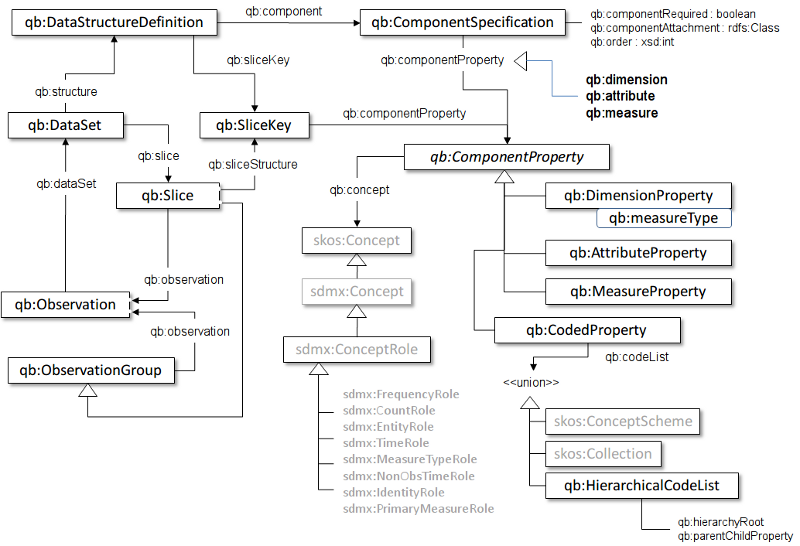
\includegraphics[width=0.8\textwidth]{img/qbstructure.png}
\caption{The Data Cube Vocabulary structure (Source: \cite{Cyganiak:14:TRD})}
\label{qbstructureimg}
\end{figure}

TODO SKOS

% The SKOS Simple Knowledge Organization System is the most reused LOD vocabulary for representation of code lists and hierarchies
% especially fitting for representing possible dimension values

% There are two main building blocks in SKOS. First, there is the skos:ConceptScheme class, representing the code list itself. Then, there is the skos:Concept class, representing the individual code list items.

\begin{figure}[h]
\begin{lstlisting}[language = turtle, caption={SKOS}, label={turtleexample},captionpos=b ,escapeinside={(*@}{@*)}]
pk:PensionKindScheme a skos:ConceptScheme ; 
    skos:prefLabel "Kinds of pensions"@en .
pkr:PK_VM a skos:Concept, pk:PensionKind ;
    skos:prefLabel "widower's pension"@en ;
    skos:inScheme pk:PensionKindScheme ;
    skos:notation "PK_VM" ;
    skos:altLabel "VM"@cs .
\end{lstlisting}
\end{figure}

